\chapter{Estado del arte} \label{chap:estadoarte}
\chapterimage{figuras/ImagenesPortada/PortadaEArte.jpg}
\hrule
\vspace{3mm}

Una vez se han repasado los aspectos generales que se buscan para este proyecto conviene hacer un estudio de la situación actual de modelos comerciales o de investigación con los que se puedan encontrar sinergias 
\\

De esta manera este capítulo hace un repaso de diferentes soluciones destinadas al soporte y posicionamiento de monitores, ordenadores o tablets. Además se hace referencia también a modelos de brazos robóticos específicamente destinados a la asistencia en entornos de usuarios. Dentro de todas las soluciones comerciales se centrará el estudio en las que están específicamente pensadas para su instalación en entornos médicos siempre que sea posible.
\\

Según el apoyo así como los tipos de grados de libertad hay diferentes configuraciones posibles, en este capítulo se verán algunos modelos concretos de cada caso evaluando sus características, ventajas e inconvenientes de los mismos de forma que se pueda generalizar a modelos equivalentes. De igual manera se podrán encontrar modelos motorizados y modelos sin motorizar, clasificación por la que serán agrupados a continuación.
\\

\section{Soportes articulados sin motorizar}

Dentro del grupo de soportes articulados sin motorizar se pueden clasificar según el tipo de anclaje que tienen, ya se enganchen al techo, pared, suelo, etc.
\\

Dentro de cada tipo de anclaje los soportes comerciales disponibles son bastante parecidos por lo que se presentará un modelo concreto que encaje dentro de las dimensiones y capacidad de carga requeridas para la aplicación que se pretende explotar para sacar conclusiones generales sobre cada tipo de soporte.

\subsection{Anclaje a la pared: Cotytech MW-M13P}

Dentro de esta gama (Cotytech MW-M*) se pueden encontrar modelos para soportar diferentes cargas. Concretamente se ha elegido el modelo con menores prestaciones y que soporta menos carga por ser suficiente para la aplicación que se pretende dar. Otros modelos pueden incluir soporte para teclado, caja y cobertura para cables y enganche a pared, entre otros, suponiendo un incremento sobre el precio de este modelo. Obtenida de \cite{CotytechMWM13P:2018} tenemos información relevante que se resume a continuación:

\begin{minipage}{0.35\textwidth}
	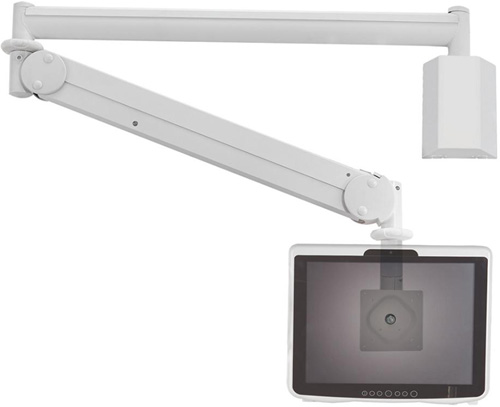
\includegraphics[width=\linewidth]{figuras/Imagenes_EstadoArte/Cotytech_MW-M13P.jpg}
\end{minipage}
\begin{minipage}{0.65\textwidth}\raggedright
	\hspace{1cm}
	\begin{itemize}
		\item Tipo de anclaje: Anclaje a la pared.
		\item Tipo de articulación: Articulaciones rotacionales.
		\item Capacidad de carga: entre $1kg$ y $6kg$.
		\item Extensión máxima: $185.7cm$.
		\item Número de grados de libertad: 5.
		\item Ángulos articulaciones: $370^o$ (brazo posición), $270^o$ (muñeca posición), $180^o$ (pared) $^1$. %fake footnote
		\item Ángulos de orientación: Tilt: $20^o$/- $35^o$ (muñeca orientación) y $20^o$/- $60^o$ (brazo orientación).
		\item Peso del soporte: $4.76 kg$.
		\item Precio estándar: 686.98\euro. $^2$. %fake footnote
	\end{itemize}
\end{minipage}

\begin{minipage}{1\textwidth}
	\footnotesize{$^1$En la imagen se pueden ver tres puntos articulados diferenciados, el punto que se fija a la pared con un grado de libertad, el punto central del brazo, que tiene dos grados de libertad (se separarán entre orientación y posición, aunque su efecto no está desacoplado)y la muñeca, que incluye la articulación que se aprecia justo encima de la pantalla como la rotacional sobre la que queda enganchada la misma (con una clasificación análoga al caso intermedio).}
	
    \footnotesize{$^2$Precio a pasado a Euros según el cambio oficial en el día consultado.}
\end{minipage}

 Paralelamente a este modelo la marca Cotytech tiene una versión que, manteniendo el mismo esquema de mecánico, permite un anclaje al techo: el modelo CM-M13 visto en \cite{CotytechCMM13:2018} con un coste de 853.06\euro.

\subsection{Anclaje al techo: Titan Elite T2EQ-C8X5}

 Concretamente se ha tomado el modelo con la montura doblada hacia arriba para un anclaje en el techo. La siguiente información constituye un resumen con los puntos más importantes vistos en \cite{TitanElite:2018}:

 \begin{minipage}{0.35\textwidth}
 	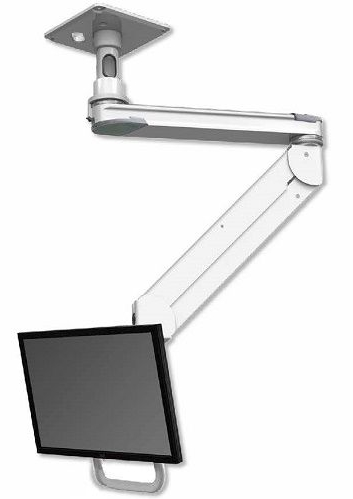
\includegraphics[width=\linewidth]{figuras/Imagenes_EstadoArte/T2EQ.jpg}
 \end{minipage}
 \begin{minipage}{0.65\textwidth}\raggedright
 	\hspace{1cm}
 	\begin{itemize}
 		\item Tipo de anclaje: Anclaje al techo.
 		\item Tipo de articulación: Articulaciones rotacionales.
 		\item Capacidad de carga: hasta $12.7kg$ en diferentes configuraciones.
 		\item Extensión máxima: $106cm$ (la longitud vertical del anclaje al techo variará según se elija al comprar).
 		\item Número de grados de libertad: 5.
 		\item Ángulos articulaciones: $360^o$ para las tres primeras articulaciones que rotan sobre el eje horizontal.
 		\item Ángulos de orientación: Tilt: $50^o$.
 		\item Peso del soporte: $9kg$.
 		\item Precio estándar: 628.30\euro.
 	\end{itemize}
 \end{minipage}
 \\

 Este mismo modelo cuenta con diferentes enganches y longitudes de los tubos que permiten anclarlo al suelo, al techo o a la pared indistintamente.

\subsection{Anclaje a una mesa o superficie de trabajo: Ergotron LX Sit-Stand Desk Arm}

 De entre la gama incluida en los modelos de Ergotron LX se ha elegido aquel que tenía unas dimensiones más ajustadas a las necesidades reales. En general el resto de la gama y otros soportes similares tienen unas dimensiones más reducidas. Resumidas de \cite{LXSitStand:2018} y \cite{LXSitStandWeb:2018} se encuentran a continuación las principales características del modelo:

 \begin{minipage}{0.35\textwidth}
 	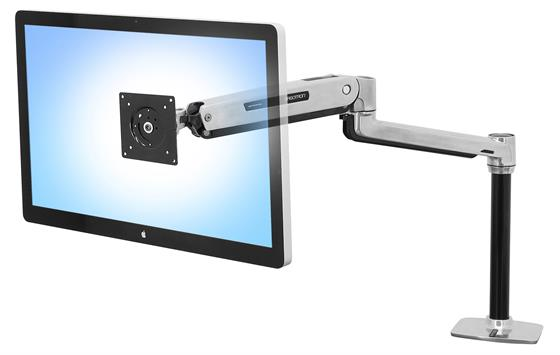
\includegraphics[width=\linewidth]{figuras/Imagenes_EstadoArte/LX_Sit-Stand_Desk_Arm.jpg}
 	\\

 	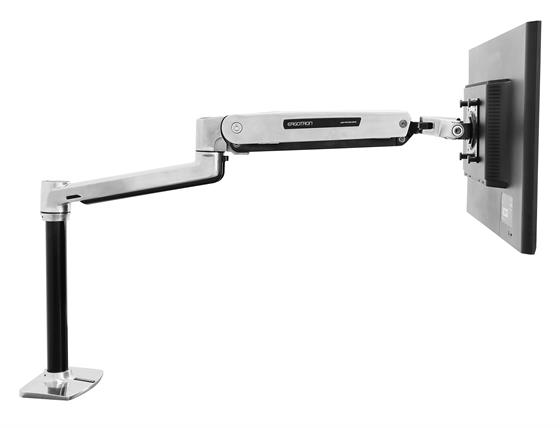
\includegraphics[width=\linewidth]{figuras/Imagenes_EstadoArte/LX_Sit-Stand_Desk_Arm_2.jpg}
 \end{minipage}
 \begin{minipage}{0.65\textwidth}\raggedright
 	\hspace{1cm}
 	\begin{itemize}
 		\item Tipo de anclaje: Anclaje a una mesa, camilla o similar.
 		\item Tipo de articulación: Primera articulación prismática, resto rotacionales.
 		\item Capacidad de carga: hasta $11.3kg$.
 		\item Extensión máxima: se puede variar hasta $36cm$ en altura (articulación prismática, esta es susceptible de ser modificada para ajustarla a otras alturas) y alcanza una extensión de $84cm$
 		\item Número de grados de libertad: 6 (una prismática y cinco rotacionales).
 		\item Ángulos articulaciones: $180^o$ la primera articulación, fija al anclaje; $360^o$ a mitad del brazo y $180^o$ en la muñeca.
 		\item Ángulos de orientación: Tilt: (giro sobre el eje medio horizontal de la pantalla) $75^o$; Pan (eje perpendicular a la pantalla): $360^o$.
 		\item Peso del soporte: $8.9kg$.
 		\item Precio estándar: 247.00\euro – 299.00\euro dependiendo de la tienda y configuración.
 	\end{itemize}
 \end{minipage}
 \\

 \vspace{0.1cm}
 Este mismo modelo cuenta con diferentes enganches y longitudes de los tubos que permiten anclarlo al suelo, al techo o a la pared indistintamente.

 \subsection{Consideraciones generales sobre los soportes no motorizados}
 Los modelos vistos hasta ahora presentan un rango de movimientos muy amplio, están certificados y preparados para su uso en entornos hospitalarios además de estar destinados precisamente al soporte de monitores. En todos los casos la capacidad de carga excede con creces la que se estima necesaria en este proyecto por lo que todas las opciones podrían ser válidas.
 \\

 Aunque cuentan con puntos bastante favorables se trata de productos cerrados sobre los cuales sería complicado integrar actuadores y sensores de manera adecuada, segura y en última instancia, elegante. Además el rango de precios en el que se encuentran es bastante elevado.

\section{Soportes articulados motorizados}

Se centrará este apartado en los modelos que se pueden ver en \cite{maiormover:2018}, como por ejemplo el MaiorFlip 900.

\begin{minipage}{0.35\textwidth}
   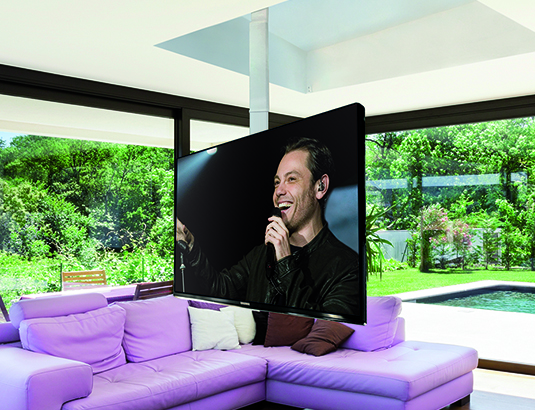
\includegraphics[width=\linewidth]{figuras/Imagenes_EstadoArte/not_valid_1.jpg}
\end{minipage}
\begin{minipage}{0.65\textwidth}\raggedright
   \hspace{1cm}
   \begin{itemize}
       \item Tipo de anclaje: Anclaje al techo.
       \item Tipo de articulación: Primera articulación rotacional, segunda prismática y tercera rotacional.
       \item Capacidad de carga: máximo de $28kg$.
       \item Extensión máxima: Descenso de hasta $68cm$
       \item Número de grados de libertad: 3 (una prismática y dos rotacionales).
       \item Ángulos articulaciones: Primera rotación giro de hasta $90^o$; articulación prismática con un alcance de $68cm$ con una capacidad de giro de la articulación final de $360^o$.
       \item Peso del soporte: $35kg$.
       \item Precio estándar: Bajo demanda.
   \end{itemize}
\end{minipage}
\\

 \vspace{0.1cm}
Otros modelos que se pueden encontrar presentan unas características similares:

\begin{minipage}{0.5\textwidth}
   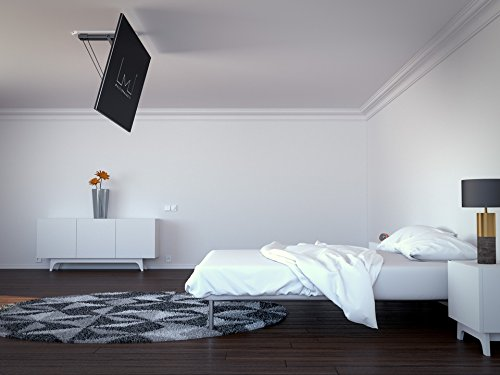
\includegraphics[width=0.8\linewidth]{figuras/Imagenes_EstadoArte/not_valid_2.jpg}
\end{minipage}
\begin{minipage}{0.5\textwidth}
   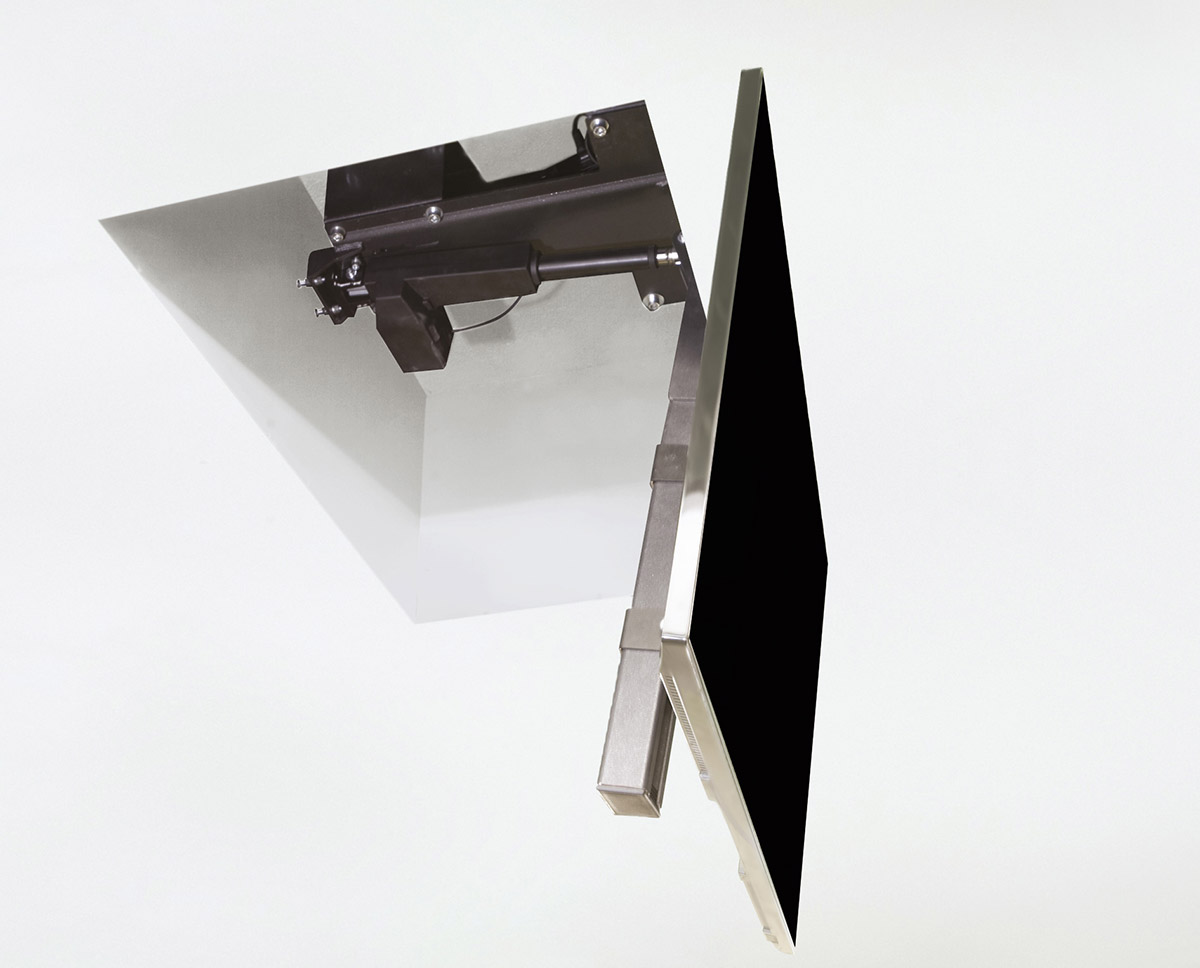
\includegraphics[width=0.8\linewidth]{figuras/Imagenes_EstadoArte/not_valid_3.jpg}
\end{minipage}
 \subsection{Consideraciones generales sobre los soportes motorizados}

    Este tipo de soportes están principalmente pensados para motorizar televisores de gran tamaño con unos rangos de movimiento bastante limitados. No son aptos para la aplicación que se pretende dar puesto que no permiten su posicionamiento a una distancia adecuada del usuario.

\section{Brazos robóticos para asistencia de pacientes}

	En general para el propósito que se plantea en este proyecto se podría adaptar una solución robótica comercial implementando una interfaz entre la tablet y el controlador del brazo. En esta sección se presentan algunos modelos de brazos robóticos especialmente pensados como robots asistenciales, preparados para una interacción directa con pacientes en entornos hospitalarios o caseros \completarCon{not the word...}.

 \subsection{JACO 3 fingers, Kinova robotics}
	 Pertenece a la línea de productos de Kinova robotics especialmente diseñados como robots asistenciales. Están pensados para una interacción directa con el paciente o usuario de forma que pueda convertirse en una extensión del mismo proporcionándole una mayor independencia. Entre las características descritas en \cite{Jaco:2018} y \cite{JacoWeb:2018} podemos recoger las siguientes más relevantes:
     \\

	  \begin{minipage}{0.35\textwidth}
	  	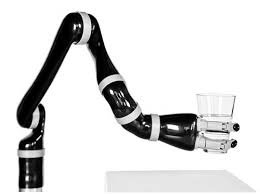
\includegraphics[width=\linewidth]{figuras/Imagenes_EstadoArte/jaco-3-finger.jpg}
	  \end{minipage}
	  \begin{minipage}{0.65\textwidth}\raggedright
	  	\hspace{1cm}
	  	\begin{itemize}
	  		\item Tipo de anclaje: Adaptativo a una mesa, silla de ruedas, etc
	  		\item Tipo de articulación: 6 grados de libertad rotacionales
	  		\item Capacidad de carga: entre $1.8kg$ y $1.6kg$ dependiendo de la versión elegida (con tres dedos tiene una capacidad menor).
	  		\item Extensión máxima: alcanza $90cm$.
	  		\item Número de grados de libertad: 6.
	  		\item Ángulos de posición: Rotación continua en las articulaciones.
	  		\item Ángulos de orientación: $55^o$ en la muñeca.
	  		\item Peso del brazo: $5.7kg$.
	  		\item Precio estándar: desde 34900\euro.
	  	\end{itemize}
	  \end{minipage}
	  \\

	  \vspace{0.1cm}

      Este modelo concreto, Jaco, viene en dos formatos pudiendo tener dos o tres dedos en el manipulador de su extremo.
      \\

	  De esta marca se puede adquirir también el modelo MICO con algo menos de alcance ($70cm$) como se ve en \cite{Mico:2018}. Los grados de libertad ofertados varían entre 4 y 7, se ha optado por tomar una solución lo más parecida a la requerida.

 \subsection{Brazo Multi-manipulador de la Universidad de Pamplona}

    Dejando de lado el ámbito puramente comercial se encuentran proyectos que es interesante repasar. En \cite{Marquez:2013} se describe un modelo diseñado específicamente como robot asistencial con capacidad de cambiar, de forma autónoma, entre diferentes manipuladores disponibles como pueden ser una cuchara, un tenedor, un cuenco, entre otros.
    \\

     \begin{minipage}{0.35\textwidth}
       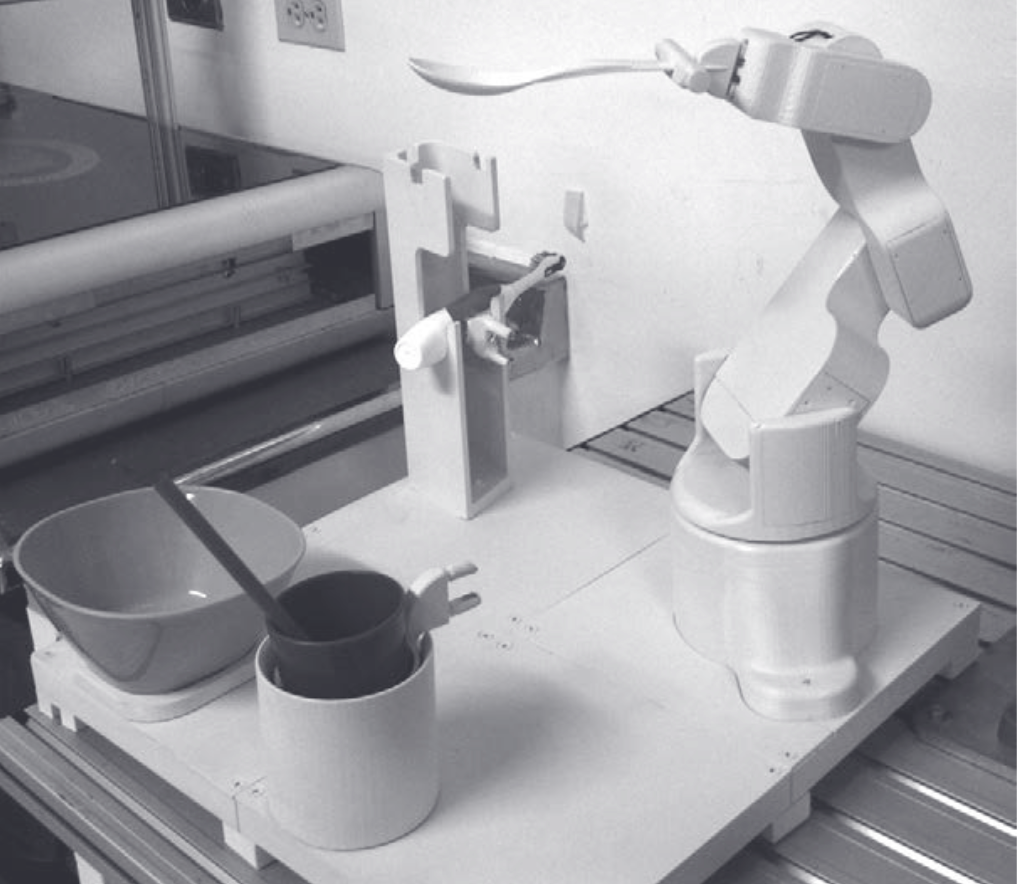
\includegraphics[width=\linewidth]{figuras/Imagenes_EstadoArte/UPamplona.png}
     \end{minipage}
     \begin{minipage}{0.65\textwidth}\raggedright
       \hspace{1cm}
       \begin{itemize}
           \item Tipo de anclaje: Lleva su propia plataforma sobre la que se monta
           \item Tipo de articulación: 4 grados de libertad rotacionales
           \item Capacidad de carga: manipuladores que adjunta.
           \item Extensión máxima: alcanza Superficie de trabajo de 40cm x 40cm.
           \item Número de grados de libertad: 4.
           \item Actuadores: Dynamixel AX-12
           \item Precio estándar: proyecto no comercial.
       \end{itemize}
     \end{minipage}
     \\

     \vspace{0.1cm}

     Es interesante destacar que aunque no se aportan demasiados datos sobre el modelo (peso del modelo, capacidad de giro de sus articulaciones, etc) si presenta un estudio completo de su aceptación así como facilidad de uso. Un sistema intuitivo es más fácilmente aceptado por los usuarios, a los cuales les será más fácil empezar a hacer uso de las facilidades que ofrece un robot de este tipo.
     \\

     Los actuadores que utiliza son de la gama de Dynamixel, una serie de servo motores muy versátiles aunque sin demasiada carga útil una vez montados sobre las articulaciones.

 \subsection{Brazo robótico para personas con movilidad reducida}

    Continuando con modelos de un ámbito más académico se encuentra el modelo descrito en \cite{Hideyuki:2010}. Se trata de un modelo plegable que puede ser almacenado o transportado dentro de una maleta de forma sencilla. Viene con un manipulador en forma de manopla que permite agarres de una amplia gama de objetos. También pensado para la asistencia de personas con movilidad reducida ha sido principalmente testeado para administrar alimentos y bebidas.
    \\

     \begin{minipage}{0.35\textwidth}
       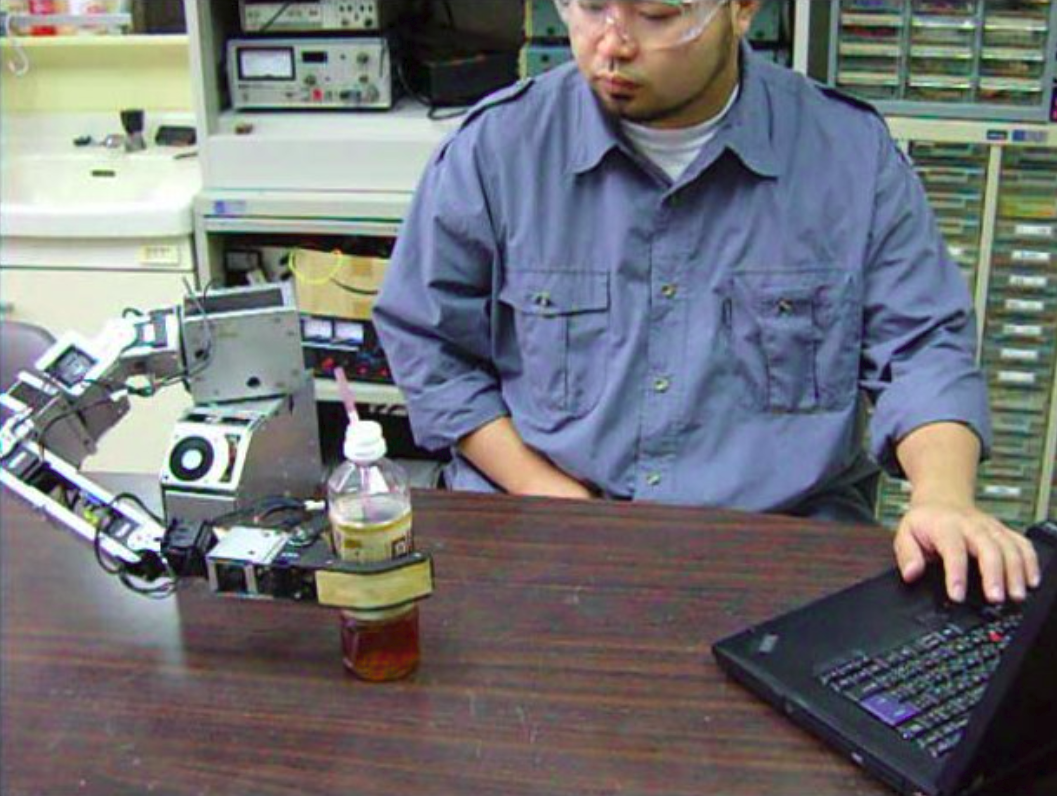
\includegraphics[width=\linewidth]{figuras/Imagenes_EstadoArte/Tokyo.png}
     \end{minipage}
     \begin{minipage}{0.65\textwidth}\raggedright
       \hspace{1cm}
       \begin{itemize}
           \item Tipo de anclaje: Sin determinar.
           \item Tipo de articulación: 7 grados de libertad rotacionales
   	  		\item Extensión máxima: alcanza $71cm$.
   	  		\item Número de grados de libertad: 7.
   	  		\item Peso del brazo: $5kg$ con dos baterías.
   	  		\item Precio estándar: proyecto no comercial.
       \end{itemize}
     \end{minipage}
     \\

     \vspace{0.1cm}
 \subsection{Consideraciones generales sobre los brazos robóticos}
    Aunque entre los modelos descritos sería fácil encontrar uno válido para la aplicación que se pretende dar, la mayoría de modelos comerciales (en los casos académicos se desconoce el precio que rondaría en caso de convertirse en producto comercial) tienen unos precios elevados que dificultarían su aplicación a gran escala.
    \\

    Estos modelos, aunque estando diseñados específicamente para entornos de interacción directa con usuarios no justifican las medidas de seguridad que se tienen en cuenta para evitar daños a los mismos. En última instancia en los diseños y prototipos encontrado no se pueden apreciar diferencias en el diseño de los mismos con modelos industriales (más allá de tamaño o peso).
